\documentclass[UTF8]{ctexart}
\usepackage{graphicx}
\usepackage[colorlinks,linkcolor=black]{hyperref}
\usepackage{listings, geometry, amsmath}
\geometry{left=3cm,right=3cm,top=3cm,bottom=4cm}
\usepackage[colorinlistoftodos]{todonotes}
\lstset{ % 代码高亮
	backgroundcolor=\color{white},   % choose the background color
	basicstyle=\footnotesize\ttfamily,        % size of fonts used for the code
	columns=fullflexible,
	numbers=left,                    % where to put the line-numbers; possible values are (none, left, right)
	numbersep=0.5em,		% how far the line-numbers are from the code
	breaklines=true,                 % automatic line breaking only at whitespace
	captionpos=t,                    % sets the caption-position to bottom
	tabsize=4,
	frame = single,
	framexleftmargin=2em,
	commentstyle=\color{mygreen},    % comment style
	escapeinside={\%*}{*)},          % if you want to add LaTeX within your code
	keywordstyle=\color{blue},       % keyword style
	stringstyle=\color{mymauve}\ttfamily,     % string literal style
	rulecolor=\color{black},
	identifierstyle=\color{red},
	language=python,
	showtabs = false,
	showstringspaces = false,
	showspaces = false,
}

\usepackage{setspace} %行间距
\onehalfspacing

\addtolength{\parskip}{.4em} %段间距

\usepackage{fancyhdr} %页眉页脚
\pagestyle{fancy}
\lhead{}
\chead{时间序列分析B 2024春}
\rhead{}
\lfoot{}
\cfoot{}
\rfoot{\thepage}
\renewcommand{\headrulewidth}{0.4pt}
\renewcommand{\headwidth}{\textwidth}
\renewcommand{\footrulewidth}{0pt}

\ctexset{section = {format = \raggedright\Large\bfseries,}} %标题左对齐

%%%%%%%%%%%%%%%%%%%%%%%%%%%%%%%%%%%%%%%%%%%%%%%%%%%%
    \title{时间序列分析B}
    \author{JiangYiFu}
    \date{\today}

    \begin{document}
    \maketitle

    \tableofcontents    
    \newpage

\section{前言}

这份复习总结是我在准备期末考试时完成的,前面几章对应课本的第一/二/三/八章节,也就是考试要求的全部章节,内容基本是我在复习过程中对课本的摘录,如果你对课本完全不熟悉可以稍微看看.最后一个章节是对考试内容的具体总结,基本选自往年真题,希望快速备考的同学建议直接看最后一章.时2024春,时间序列分析B常被诟病简单且考试题目类型雷同,不知道以后会不会进行课程改革,故此资料仅作参考.欢迎后人对源文件进行修改.

\section{金融时间序列基础知识}

简单收益率$R_t$,多期简单收益率$R_t [k]$,\[1+R_t [k]=\prod_{j=0}^{k-1}(1+R_{t-j})\]

\hspace*{\fill}

连续复合,理解为利息计算时间由1年转变为每时每刻都在结息(即结算时间无穷小,转化为极限计算,得到的结果是理论上利息最高值),此时资产净值为,\[A=C \cdot exp(r\times n)\]其中C是初始资产,r是年利率,n是年数.

\hspace*{\fill}

资产的简单毛收益率的自然对数称为1连续复合收益率或对数收益率,\[r_t = \ln(1+R_t)=\ln(\dfrac{P_t}{P_{t-1}})\],注意到其多期情况计算的简便性,\[r_t[k]=\sum_{i=0}^{k-1}r_{t-i}\]

\hspace*{\fill}

随机变量的矩,一个连续型随机变量X的$l$阶矩定义为,\[m_l '=E(X^{l})=\int_{-\infty}^{\infty}x^{l}f(x)dx\],一阶矩称为X的均值或期望,记为$\mu_x$,X的$l$阶中心矩定义为,\[m_l =E((X-\mu_x)^{l})=\int_{-\infty}^{\infty}(x-\mu_x)^{l}f(x)dx\]二阶中心矩称为X的方差,记为$\sigma_x^2$,三阶中心矩度量X关于其均值的对称性,而四阶中心矩度量X的尾部,标准化的三阶矩称为偏度,标准化的四阶矩称为峰度.\[S(x)=E[\dfrac{(X-\mu_x)^3}{\sigma_x^3}],K(x)=E[\dfrac{(X-\mu_x)^4}{\sigma_x^4}]\]

\hspace*{\fill}






\section{线性时间序列分析及其应用}

把资产收益率(如股票的对数收益率$r_t$)看成随时间推移而形成的一族随机变量,我们就有了一个时间序列$\{r_t\}$.特别地,所研究的变量与其过去值的相关系数成为线性时间序列分析的焦点.这些相关系数称为序列相关系数或自相关系数.

\hspace*{\fill}

平稳性是时间序列分析的基础.如果对所有的$t$,任意正整数$k$和任意$k$个正整数$(t_1,...,t_k),(r_{t_1},...,r_{t_k})$的联合分布与$(r_{t_1+t},...,r_{t_k+t})$的联合分布是相同的,那么时间序列$\{r_t\}$称为严平稳的.如果$r_t$的均值与$r_t$和$r_{t-l}$的协方差不随时间而改变,其中$l$是任意整数,那么时间序列$\{r_t\}$称为弱平稳的.\[Cov(X,Y)=E[(X-E[X])(Y-E[Y])]=E[XY]-E[X]E[Y]\]协方差为0的两个随机变量称为是不相关的.

\hspace*{\fill}

两个随机变量X和Y的相关系数定义为\[\rho_{x,y}=\dfrac{Cov(X,Y)}{\sqrt{Var(X)Var(Y)}}\]考虑弱平稳收益率序列$r_t$.当我们考虑$r_t$与它的过去值$r_{t-i}$的线性相依关系时,可以把相关系数的概念推广到自相关系数(ACF).$r_t$与$r_{t-l}$的相关系数称为$r_t$的间隔为$l$的自相关系数,通常记为$\rho_l$,注意到方差和协方差之间的联系.\[\rho_l=\dfrac{Cov(r_t,r_{t-l})}{Var(r_t)}=\dfrac{\gamma_l}{\gamma_0}\]

\hspace*{\fill}

如果$\{r_t\}$是一个具有有限均值和有限方差的独立同分布随机变量序列,那么时间序列$\{r_t\}$称为一个白噪声序列.特别地,如果$r_t$还服从均值为0,方差为$\sigma^{2}$的正态分布,则称这个序列为高斯白噪声.

\hspace*{\fill}

时间序列$\{r_t\}$称为线性序列,如果它能写成\[r_t=\mu + \sum_{i=0}^{\infty}\psi_i a_{t-i},\]其中$\mu$是$r_t$的均值,$\psi_0=1$,$\{a_t\}$是白噪声序列.我们主要关心的是$a_t$为连续型随机变量的情形.\[E(r_t)=\mu,Var(r_t)=\sigma_{a}^2\sum_{i=0}^{\infty}\psi_i^2\]$r_t$的间隔为$l$的自协方差为\[\gamma_l=\sigma_{a}^2\sum_{j=0}^{\infty}\psi_j \psi_{j+l}\]

\hspace*{\fill}

\[r_t=\phi_0+\phi_1 r_{t-1}+a_t,\]一阶自回归(AR)模型,或者简称AR(1)模型.其中$a_t$是均值为0的白噪声序列.由该模型可以推得,\[E(r_t|r_{t-1})=\phi_0+\phi_1 r_{t-1},Var(r_t|r_{t-1})=Var(a_t)=\sigma_{a}^{2}\]

\hspace*{\fill}

AR(1)模型的弱平稳性的充分必要条件$\Longrightarrow$ $|\phi_1|<1$.(思考证明过程)

\hspace*{\fill}

AR(2)模型形如\[r_t=\phi_0+\phi_1 r_{t-1}+\phi r_{t-2}+a_t.\]利用与AR(1)情形相同的方法,我们知道,只要$\phi_1+\phi_2 \neq 1$,就有\[E(r_t)=\mu=\dfrac{\phi_0}{1-\phi_1-\phi_2}\]对式子进行处理得到\[\gamma_l = \phi_1 \gamma_{l-1}+\phi_2 \gamma_{l-2}\]被称为平稳AR(2)模型的矩方程.对其两端同除以$\gamma_0$,得到$r_t$的ACF的性质.

\hspace*{\fill}

上面的式子说的是:平稳AR(2)序列的ACF满足二阶差分方程\[(1-\phi_1 B-\phi_2 B^2)\gamma_l=0\]其中B是向后推移算子,即$B\gamma_l = \gamma_{l-1}$.

\hspace*{\fill}

滑动平均模型(MA),看成参数受某种限制的无穷阶AR模型.MA(1)模型的一般形式为\[r_t=c_0+a_t-\theta_1 a_{t-1}\]其中$c_0$是一个常数,$\{a_t\}$是一个白噪声序列.类似地,MA(2)模型的形式为\[r_t=c_0+a_t-\theta_1 a_{t-1}-\theta_2 a_{t-2}\]

\hspace*{\fill}

MA模型总是弱平稳的,因为它们是白噪声序列的有限线性组合,其前二阶矩是不随时间变化的.\[E(r_t)=c_0,Var(r_t)=(1+\theta_1^2+\theta_2^2+...+\theta_q^2)\sigma_a^2.\]

\hspace*{\fill}

关于定阶,MA模型---ACF(自相关函数),AR模型---PACF(偏自相关函数).

\hspace*{\fill}

自回归滑动平均(ARMA)模型,ARMA(1,1)模型\[r_t-\phi_1 r_{t-1}=\phi_0+a_t-\theta_1 a_{t-1}\]

\hspace*{\fill}

单位根非平稳序列---随机游动模型.

\hspace*{\fill}





\section{条件异方差模型}

用$r_t$表示某资产在$t$时刻的对数收益率,波动率研究的基本思想是,序列$\{r_t\}$是序列不相关或低阶序列相关,但是它是相依序列.

\hspace*{\fill}

本章的条件异方差模型就是用来描述$\sigma_t^2$的演变的.$\sigma_t^2$随时间变化的方式可以用不同的波动率模型来表示.条件异方差性建模就是对时间序列模型增加一个动态方程,来刻画资产收益率的条件方差随时间的演变规律.

\hspace*{\fill}

ARCH模型,其思想是:1.资产收益率的扰动$a_t$是序列不相关的,但不是独立的.2.$a_t$的不独立性可以用其延迟值的简单二次函数来描述.\[a_t=\sigma_t \varepsilon_t,\sigma_t^2=\alpha_0+\alpha_1 a_{t-1}^2+...+\alpha_m a_{t-m}^2\]其中$\{\varepsilon_t\}$是均值为0,方差为1的独立同分布随机变量序列.

\hspace*{\fill}

GARCH模型

     \begin{figure}[h]
         \centering
         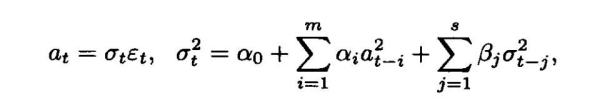
\includegraphics[scale=0.45]{images9.png}
     \end{figure}





\section{多元时间序列分析及其应用}


多元时间序列包含多个一元时间序列作为其分量.







\section{考试重点-真题}

     \begin{figure}[h]
         \centering
         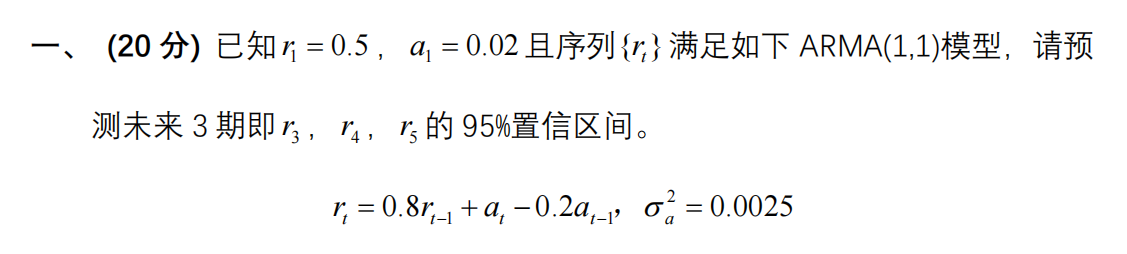
\includegraphics[scale=0.35]{images1.png}
     \end{figure}

考点解析:线性时间序列预测相关

\hspace*{\fill}

设$\hat{r}_h(l)$为$r_(h+l)$的最小均方预测.以AR(p)模型为例子,计算向前1步预测,即计算条件期望\[\hat{r}_h(1)=\phi_0+\sum_{i=1}^{p}\phi_i r_{h+1-i}\]对应的误差为\[e_h(1)=r_{h+1}-\hat{r}_h(1)=a_{h+1}.\]从而,向前1步预测误差的方差为$Var[e_h(1)]=Var(a_{h+1})=\sigma_a^2$,当$a_t$服从正态分布时,则$r_{h+1}$的$95\%$的向前1步区间预测是$\hat{r}_h(1)\pm 1.96 \times \sigma_a.$而对于向前2步预测,处理方式相似,唯一需要注意的是在计算条件期望时结果中会存在向前1步预测.

\hspace*{\fill}

     \begin{figure}[h]
         \centering
         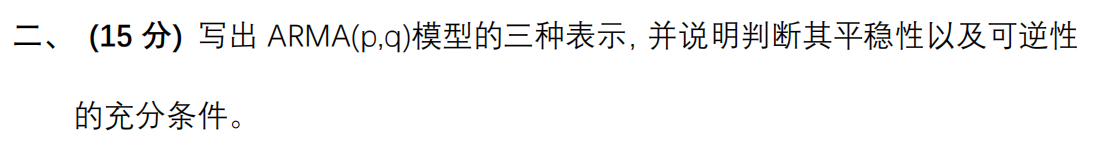
\includegraphics[scale=0.35]{images2.png}
     \end{figure}

考点解析:模型形式默写,平稳性可逆性等性质证明.

\hspace*{\fill}

AR(p)模型\[r_t=\phi_0+\phi_1 r_{t-1}+...+\phi_p r_{t-p}+a_t,\]这里的$\{a_t\}$是均值为0,方差为$\sigma_a^2$的白噪声序列.

\hspace*{\fill}

考虑AR(1)模型的弱稳定性的充分必要条件.回想弱稳定性的定义:均值+方差+协方差.\[E(r_t)=\mu,Var(r_t)=\gamma_0,Cov(r_t,r_{t-j})=\gamma_j\]

     \begin{figure}[h]
         \centering
         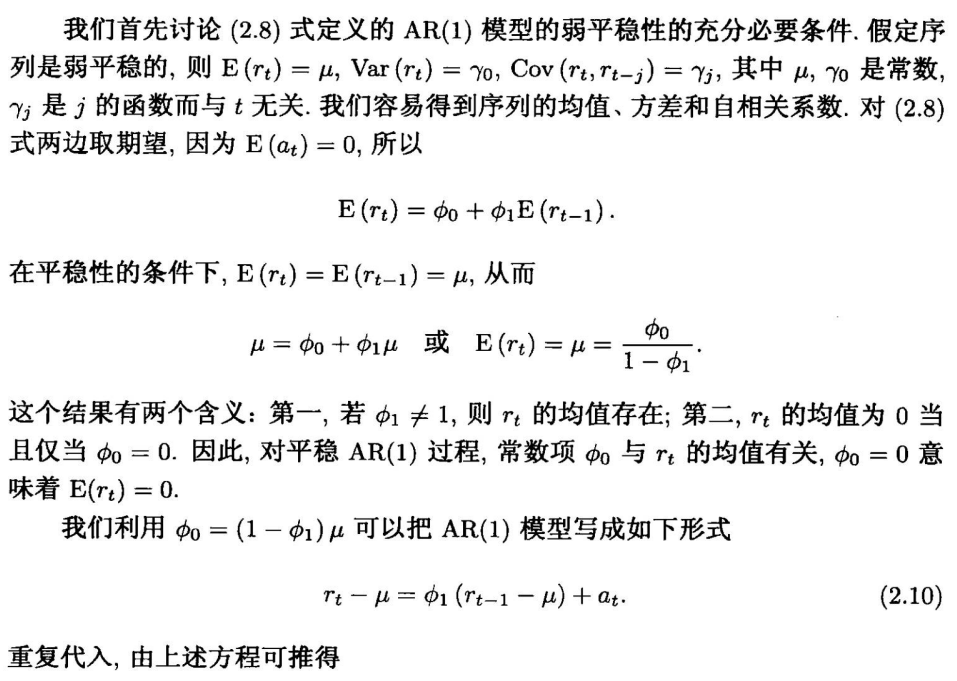
\includegraphics[scale=0.28]{images3.png}
     \end{figure}

     \begin{figure}[h]
         \centering
         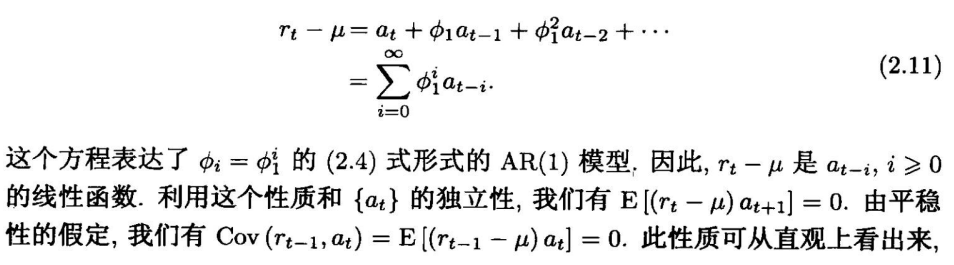
\includegraphics[scale=0.28]{images4.png}
     \end{figure}

     \begin{figure}[h]
         \centering
         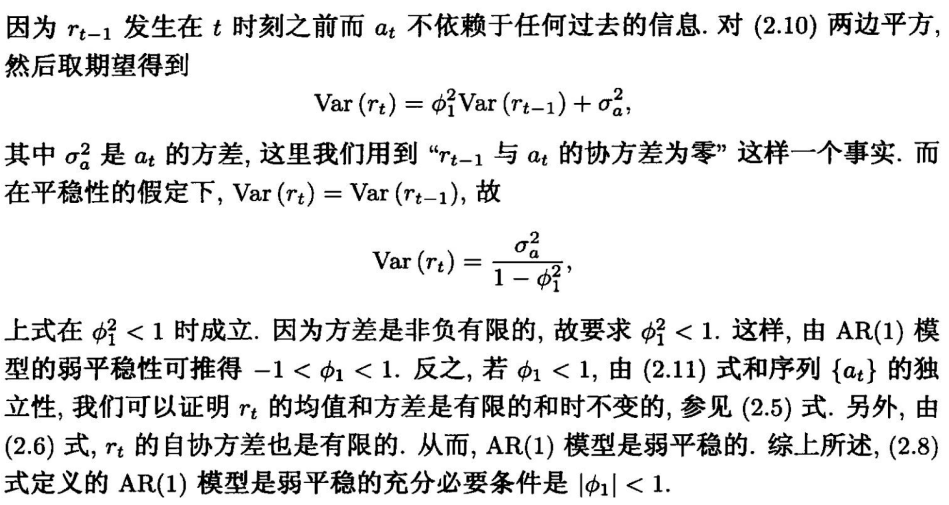
\includegraphics[scale=0.28]{images5.png}
     \end{figure}

\hspace*{\fill}

MA(q)模型\[r_t=c_0+a_t-\theta_1 a_{t-1}-...-\theta_q a_{t-q}.\]

\hspace*{\fill}

ARMA(p,q)模型\[r_t=\phi_0+\sum_{i=1}^{p}\phi_i r_{t-i}+a_t-\sum_{i=1}^{q}\theta_i a_{t-i},\]如果利用向后推移算子,该模型可以写成\[(1-\phi_1 B-...-\phi_p B^p)r_t=\phi_0+(1-\theta_1 B-...-\theta_q B^q)a_t.\]我们用两个多项式比的级数展开式(长除法).

     \begin{figure}[h]
         \centering
         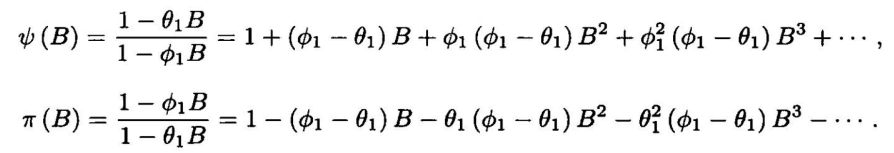
\includegraphics[scale=0.35]{images6.png}
     \end{figure}

     \begin{figure}[h]
         \centering
         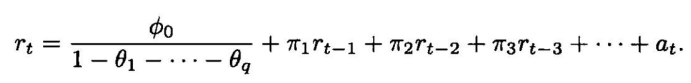
\includegraphics[scale=0.4]{images7.png}
     \end{figure}

     \begin{figure}[h]
         \centering
         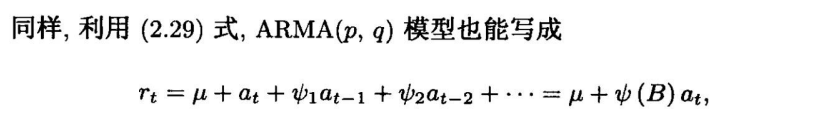
\includegraphics[scale=0.42]{images8.png}
     \end{figure}

\hspace*{\fill}

     \begin{figure}[h]
         \centering
         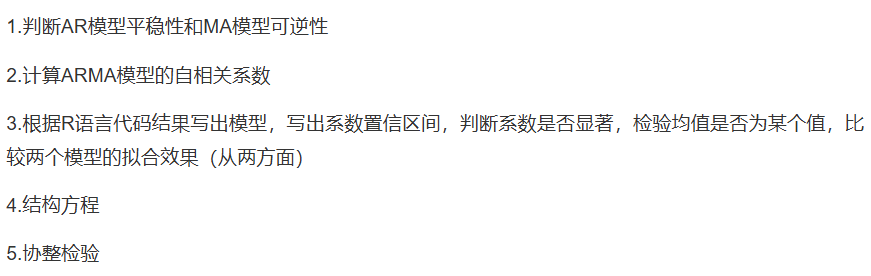
\includegraphics[scale=0.42]{images10.png}
     \end{figure}

\hspace*{\fill}

     \begin{figure}[h]
         \centering
         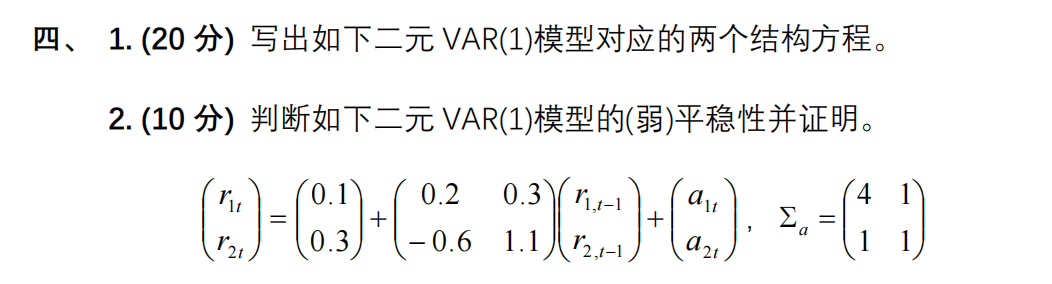
\includegraphics[scale=0.32]{images11.png}
     \end{figure}










    \end{document}